
\documentclass[twoside,leqno,twocolumn]{article}
\usepackage{ltexpprt} 

\usepackage{algorithmic}
\usepackage{algorithm}
%\usepackage{algorithmicx}
\usepackage{listings}
\usepackage{color}
\usepackage{xspace}
\usepackage{graphicx}
\usepackage{caption}
\DeclareCaptionType{copyrightbox} % Temporary hack to use the caption package
\usepackage{subcaption}
\usepackage{alltt}
\usepackage{balance}
\usepackage{hyperref}
\usepackage{paralist}
%\usepackage[top=0.75in, bottom=1in, left = 0.68in, right=0.68in]{geometry}
\usepackage{cite}
\usepackage{amsmath}
\usepackage{url}


\newcommand{\ceg}[1]{{\textcolor{green}{#1 --- CEG}}}
\newcommand{\dzw}[1]{{\textcolor{magenta}{#1 --- CEG}}}
\newcommand{\eat}[1]{}
\newcommand{\qgram}{$q$-gram\xspace}
\definecolor{gray}{rgb}{0.5,0.5,0.5}
\newcommand{\added}[1]{\textcolor{blue}{#1}}
\newcommand{\changed}[1]{\textcolor{red}{#1}}
\newcommand{\removed}[1]{\textcolor{gray}{#1}}









\begin{document}

\title{A Proposal Optimizer for Sampling-Based Entity Resolution}

\author{%
Christan Earl Grant\thanks{Datascience Research Lab, University of Florida; \url{cgrant@cise.ufl.edu}} 
\and 
Daisy Zhe Wang\thanks{Datascience Research Lab, University of Florida; \url{daisyw@cise.ufl.edu}}}

\date{}

\maketitle




\begin{abstract}
%\small\baselineskip=9pt
Increasingly, organizations have employed methods to understand unstructured text across the web.
Entity resolution is used to identify mentions in large, streaming text corpora.
Sampling-based entity resolution using Markov Chain Monte Carlo (MCMC) techniques guarantees convergence to a stationary distribution and can jump out of local optimum.
When performing entity resolution over streams of incoming data, the growing quantity of data amplifies two main issues.
First, because the sampling process is random, many iterations are wasted attempting to resolve unambiguous entities.
Second, the quadratic runtime for scoring entities becomes prohibitive for largest entities.
%When new documents are continuously updated the above issues are exacerbated.
Frequent streaming updates from the web exacerbate these difficulties.
In this paper, we discuss the creation of a proposal optimizer, in the spirit of database optimizers.
This optimizer observes the proposal updates to the entity resolution model
then makes recommendations to improve the processing and storage of the model.
We motivate the use of compression techniques to reduce the amount of processing when scoring MCMC updates proposal.
We also discuss statistical early-stopping techniques for scoring entities.
We describe our initial progress over a large entity resolution data set and
how an optimizer can improve performance when processing entity resolution streams.


\end{abstract}



\section{Introduction}

% What is the problem
The storage of user generated content within systems has introduced 
vast amounts of data.
To correctly process this data must be cleaned. 
Entity resolution is an important part of the ubiquitous cleaning task.
Entity Resolution (ER) is the problem of resolving records in
a data set that correspond the same real world entity.

% Why is the problem hard
Entity resolution is a notoriously computationally difficult problem.
Several efforts in different domains have made outstanding progress~\cite{}.
The main issues still affecting runtimes of ER systems are
twofold, first, the computation of large entities and second, excessive
computation spent resolving unambiguous entities.
Optimization that touches these critical portions is wholly understudied.
We argue that compression and approximation 
techniques can efficiently decrease the runtimes of traditional ER systems.

There is not one size fits all techniques even inside sampling algorithms~\cite{sculley2006compression}.

% What are the technical challenges and validation
Some recently, researchers have suggest methods of compressing entities.
Wick et al Heirchical \ldots

Singh et all efficient factoring % http://people.cs.umass.edu/~sameer/files/mcmcmc-emnlp12-ppt.pdf

Each of these methods has drawbacks \ldots

% How we differ
In this paper, we train a multi-class classifier to optimize the decision of
the sampling inference technique to apply.


% Our contributions
We make the following contributions

\begin{itemize}
\item We identify several techniques to speed up sampling past the baseline~\ref{}.
\item We create an optimizer to choose parameters and methods at run time~\ref{}.
\item We empirically evaluate these methods over a large data set~\ref{}.
\end{itemize}



% Links to people who used vectorization
% http://citusdata.github.io/cstore_fdw/
% http://www.drdobbs.com/parallel/parallel-in-place-merge-sort/240169094?pgno=2




\section{Background}

Entity Resolution

Blocking

The distribution of entitiy sizes


\section{Related Work}

Wick et al

Sameer Singh

Pay as you go ER




\section{Example}

In this section we discuss define the acceleration in MCMC-MH sampling for entity resolution.
We then motivate how we believe gains can be achieved given using compression, sampling acceleration methods and optimizers.

The issues we are investigating are as follows.
First, Given an Entity $e_i$ how can we create a structure with \textit{minimal total size}.
%Second, How can we incrementally add and remove items 
%from the compressed structure.
Next, how can we compute the features over a source and destination entity ($e_s$, $e_d$) 
in the \textit{smallest amount of time}.
Lastly, how do we \textit{decide} when to use each technique.


The total size of all entities in the traditional representation is:

\begin{equation}
  \text{sizeof}(\mathcal{E}) =  \sum_i c + (\text{sizeof}(\text{int}) * |e_i|),
\end{equation}
where $sizeof$ is an abstract function to compute the size of the containing object,
$c$ is a class constant and $|e_i|$ is number of mentions in the entity.

There are many compression techniques, one being we only keep the mentions an entity
that have a unique representation.
That is, if any mention token is a duplicate, we remove it.
This compressed total entity size size is:

\begin{equation}
  \text{sizeof}(\mathcal{E_\text{compressed}}) = \sum_i c + (\text{sizeof}(int) * \#(e_i) ),
\end{equation}
where $\#(e_i)$ is the cardinality of the mention tokens in entity $e_i$.
We note that when the $\#(e_i) \ll |e_i|$ it may be worth compressing this entity.


In the example data set in Figure~\ref{fig:entity-distribution} we note that
45\% percent of mentions are smaller that 100 mentions in size.
Additionally, 82\% percent of entities contain less than 1000 mentions.
These number suggest that at times we 
we can take advantage of the redundancy within
large entities and compress the entities.
(We investigate the WikiLinks corpus further in Section~\ref{sec:microbenchmark}). 






\section{Algorithms}

In this section we will describe XXX algorithms for entity sampling.
The main method we use to improve the computation speed is to reduce the
number of comparisons we make for large entity clusters.
We additionally discuss methods to improve the performance of algorithms
over time by collecting statistics from the processes.

\textbf{Naive Iterator.} This method performs pairwise comparisons by 
iterating over the mentions using the order on disk. This is the traditional
method of computing the pairwise similarity of two clusters. 

\textbf{SubSample Iterator.} This method performs uniform samples of the
mentions from the source and destination entities clusters. This method
measures the confidence of the calculated pairwise samples and stops when the
confidence exceeds a threshold of 0.95.

\textbf{Top-K SubSample Iterator.} This method uses a priority queue to sort
the mentions and only performs comparisons between the top $M$ mentions.

\textbf{Blocked Iterator.} This method performs blocking on the mentions in the
source and destination entities and takes the average gain from pairwise
comparisons inside each block. Blocks are formed arbitrarily and are of fixed
size. In database terms this method is a \emph{block nested loop} comparison.

\textbf{Blocked Subsample Iterator.} This performs a block nested loop
comparisom but it performes book keeping to only perform pairwise sampling
until we reach a confidence threshold of 0.95.

\textbf{Blocked Top-k Iterator.} This method performs a block nested loop
comparison except blocks are created by reading mentions from a priority queue.

\textbf{Blocked Top-K Subsample Iterator.} This method is a combination of the
Block subsample iterator and the blocked top-k iterator.

Further, We examine active learning techniques to adjust threshold sizes based
on statistics collected while running the algorithms.

We collect the following statistics from each training run:

Success and failure
Data set size.
Number of uniques tokens.
Average pairwise score between mentions.
Maximum pairwise score between mentions.
Minimum pairwise score between mentions.
Variance of the pairwise score between mentions.
Mention Token tfidf scores.
Cardinality of tokens in both entities.
\ceg{Generailze the feature explaination and move it to the implementation section}

Using this information we train a decision tree classsifier to minimize the 
pairwise comparisons in the score function.
The classifier is also constrained by the accuracy of the decision tree as 
approximate methods are less accurate.
More formally \ldots

The result of this classifier is two-fold.
First, we have a classifier to choose the optimal algorithm for each proposal.
Second, we have an active learning feed-back loop for algorithms with 
thresholds.
We emperically study both of these outcomes.






\section{Implementation}

In this section we first present a microbenchmark to validate our invsitgation of entity approximation and compression.
We then discuss the implementation of the compression and approximation techniques over a large real-world
cross-document coreference corpus.

\subsection{Microbenchmark}
\label{sec:microbenchmark}
To increase our intuition of early stopping techniques we simulated the MCMC proposal processes. 
We hypothesis that there was bould a clear range values where performing the
baseline cluster sampling would be faster when compared to early stopping methods.
We arrange entity clusters of increasing time and we compute the time (in clock ticks)
each proposal takes to compute the arrangement of the clusters.
The data in the clusters are disctributed uniformly and for this experiment each cluster point
was 5 dimensional.
For the baseline cluster score computation we used a pairwise calculated of the average cosine distance
with and without the mention.
To compute early stopping we set a confidence threshold to $0.8$ and the early
stopping code stopped computation when the error predition was under $20\%$.
There was no difference in the proposal choices between the baseline and the early sorting method. 

The simulations were developped in \texttt{GNU C++11} and compiled with \texttt{g++ -O3}. 
The CPU was an 8 core intel i7 with 3.2 HGz and 12 GBs of Memory.
Each arrangement was run 5 times and results averages.


Experiment Results\ldots
The result of this experiment is summarized in Figure~\ref{fig:clustering-v-early-stopping}.
On the x-axis is the number of mentions in the source and destination clusteris for each proposal. 
The y-axsis is the number of clock ticks on a log scale.

\begin{figure}
\centering
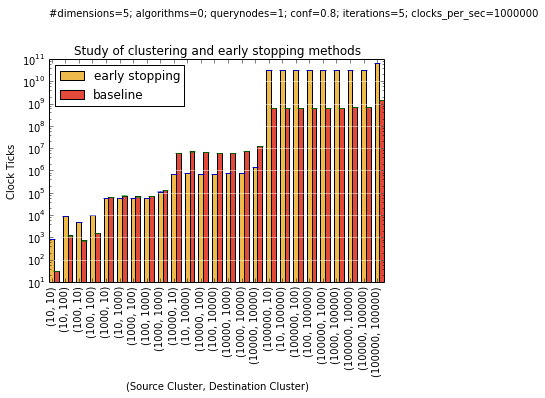
\includegraphics[width=\columnwidth, clip=true,trim=0cm 0cm 0cm 1cm]{media/clustering-v-early-stopping.png}
\caption{Comparison of baseline verses early stopping methods.}
\label{fig:clustering-v-early-stopping}
\end{figure}

We observe that for proposals with less than 100 and 1000 source and
destination mentions, the performance of the baseline proposer is better than
or almost equal to that of the more sorted early stopping method.
For proposals that contain an entity cluster with more than 10000 mentions
the early stopping method performs significantly better than the baseline method.

The optimization found in predictable code paths make simple implementations
like the baseline method attactive for small cluster sizes.
In addtion, $82\%$ of the entities in the truthed Wiki-Links data sets are less
that 1000 mentions in size and $45\%$ of the entities contain less than 100
mentions.

The results of the microbenchmark suggests that different proposal estimation techniques are useful at different times.




\subsection{Wiki Link Corpus}





\section{Evaluation}
%% TODO change to Discussion?





\section{Summary}

In this paper, we describe an initial approach for optimizing sampling for the entity resolution process.
We begin to develop an optimizer that attacks two major limitations, the size of the entities and the redundant computation.
This paper motivated the need for the optimizer and examined the feasibility of its treation.
We plan to implement the full optimizer over a large, streaming corpus, with resolved entities.
We hope to soon have a fully resolved TREC streamcorpus\footnote{\url{http://trec-kba.org/kba-stream-corpus-2014.shtml}} and examine the performance of the optimizer of that large data set.
Additionally, we hope to compare results with enterprise ER systems such as WOO~\cite{bellare2013woo}.



% TODO --- add the bibliography

\bibliographystyle{abbrv}
\bibliography{citations}

\end{document}

